\documentclass[11pt,a4paper]{article}
\usepackage[margin=25mm]{geometry}
\usepackage[T1]{fontenc}
\usepackage{mathpazo,amsmath,amssymb,graphicx,booktabs,longtable,array,caption,setspace,microtype}
\usepackage[hidelinks]{hyperref}
\usepackage{fancyhdr}
\usepackage[mathlines]{lineno}
\setstretch{1.2}
\setlength{\parskip}{4pt}
\setlength{\parindent}{0pt}
\captionsetup{font=small,labelfont=bf}
\pagestyle{fancy}\fancyhf{}\fancyhead[L]{\small GBD 2023: infertility contrasts}\fancyhead[R]{\small Additional file 1}\fancyfoot[C]{\thepage}
\setlength{\headheight}{14pt}
\setlength{\emergencystretch}{2em}
\newcommand{\ASPR}{\mathrm{ASPR}}
\title{Additional file 1: Supplementary methods and results}
\author{Companion to the Reproductive Health manuscript draft}
\date{25 October 2026}
\begin{document}\maketitle
\subsection*{Additional arithmetic definitions}
The same-population benchmark is $B_T=\sum_a P_{C,aT}(r_{C,aT}-r_{R,aT})/10^5$. It uses China's actual age distribution rather than standard weights and is not preventable burden. Age-specific contributions to the standardized difference are $w_a(r_{C,at}-r_{R,at})$. The seven published unnormalized standard weights, in ascending age order, are 0.082891, 0.078012, 0.075914, 0.073217, 0.068281, 0.061474 and 0.055113; they sum to 0.494902 before renormalization. References and outcome definitions are given in the main manuscript.
\section{Supplementary methods and results}
\renewcommand{\thetable}{S\arabic{table}}\setcounter{table}{0}
\renewcommand{\thefigure}{S\arabic{figure}}\setcounter{figure}{0}
\subsection{Decomposition of case-count changes}
We expressed the case count as $F(N,\boldsymbol f,\boldsymbol p)=N\sum_a f_a p_a$, where $N$ is the total female population aged 15--49, $f_a$ is its age distribution, and $p_a$ is age-specific prevalence as a proportion. For each factor, we averaged its marginal contribution across all six possible replacement orders between the starting and ending states. These Shapley contributions sum exactly to the observed modeled case-count change. We examined 1990--2023 and 2010--2023 for both causes in all 19 countries. Population size here refers specifically to females aged 15--49; age composition refers to redistribution within this range. The age-specific prevalence component includes epidemiological change, ascertainment and modeling changes and cannot be interpreted as a causal risk-factor contribution.

\subsection{Trends, sensitivities and forecast validation}
We fitted continuous piecewise linear models to log standardized rates, searching integer-year knot locations with zero to two knots and at least five observations per segment, counting shared boundary years in each segment. Model selection used the Bayesian information criterion, including a penalty for knot locations. Segment-specific annual percentage change was $100[\exp(\beta)-1]$; average annual percentage change (AAPC) was obtained from duration-weighted log slopes. These fits summarize modeled trajectories and are not outputs of the proprietary Joinpoint program. AR(1) generalized least-squares refits retained the OLS-selected knots; allowing up to three knots and restricting the period to 2010--2023 were additional sensitivities. Trend confidence intervals are conditional on selected knots and fixed GBD point estimates.

Reference sensitivities used age-specific country population shares fixed at 1990, excluded one reference country at a time, and restricted ages to 20--49 with renormalized weights. Following inspection of the terminal-year endometriosis increase, we added analyses ending in 2021 and 2022; these endpoint analyses were not prespecified. To evaluate numerical sensitivity to published weight rounding, we evaluated all $2^7$ combinations of perturbing unnormalized weights by $\pm0.5\times10^{-6}$. The resulting deterministic envelopes are not uncertainty intervals.

An exploratory forecasting module evaluated each Chinese age-specific prevalence series on the logit scale. Candidates were a constant-last-rate baseline, ARIMA with $p,q\in\{0,1,2\}$ and $d\in\{0,1\}$ selected by training-set corrected AIC, and additive damped-trend exponential smoothing. ARIMA candidates failing convergence were excluded. Rolling training windows contained at least 20 years and assessed horizons 1, 3 and 5; a separate last-10-year holdout assessed horizons 1--10. We specified an exploratory retention rule before running this module: at least 10\% lower mean absolute error (MAE) than the baseline in every age group in both validation schemes, with complete predictions. Future counts would additionally require compatible population projections; none were generated when validation failed. This module was not a validation against independent observed infertility data.

\begin{table}[htbp]\centering\small
\caption{Shapley decomposition of changes in China's modeled prevalent cases, thousands.}\label{tab:decomp}
\setlength{\tabcolsep}{4pt}
\begin{tabular}{llrrrr}\toprule
Cause & Period & Net change & Population size & Age composition & Prevalence\\\midrule
Endometriosis & 1990--2023 & -11.3 & -8.7 & 30.8 & -33.4 \\
Endometriosis & 2010--2023 & 6.1 & -38.4 & 7.7 & 36.8 \\
PCOS & 1990--2023 & 783.4 & -68.4 & -8.9 & 860.7 \\
PCOS & 2010--2023 & -129.8 & -414.4 & -18.2 & 302.9 \\
\bottomrule
\end{tabular}
\caption*{Population size is the female population aged 15--49; age composition is its within-range distribution; prevalence is age-specific modeled infertility prevalence. Contributions may exceed the net change and need not have the same sign. Rounding can cause small displayed discrepancies.}
\end{table}

\begin{table}[htbp]\centering\small
\caption{Restricted-age standardized YLD rates and YLD totals.}\label{tab:yld}
\setlength{\tabcolsep}{3.5pt}
\begin{tabular}{llrrrrrr}\toprule
 & & \multicolumn{2}{c}{YLDs, thousands} & \multicolumn{2}{c}{Rate per 100,000} & & \\
Cause & Year & China & Reference & China & Reference & $D$ & $RR$\\\midrule
Endometriosis & 1990 & 1.0 & 2.2 & 0.34 & 0.39 & -0.05 & 0.872 \\
Endometriosis & 2023 & 1.0 & 2.6 & 0.29 & 0.31 & -0.02 & 0.934 \\
PCOS & 1990 & 5.9 & 20.5 & 1.80 & 3.59 & -1.79 & 0.502 \\
PCOS & 2023 & 10.1 & 35.5 & 3.31 & 4.22 & -0.91 & 0.784 \\
\bottomrule
\end{tabular}
\caption*{All values are derived point estimates. YLD: years lived with disability.}
\end{table}
\begin{table}[htbp]\centering\small
\caption{Endpoint sensitivity added after inspection of terminal-year estimates.}\label{tab:endpoint}
\begin{tabular}{llrrrrr}\toprule
Cause & End year & China ASPR & Ref. ASPR & $D$ & $RR$ & $D_T-D_{1990}$\\\midrule
Endometriosis & 2021 & 43.48 & 51.93 & -8.45 & 0.837 & -5.52 \\
Endometriosis & 2022 & 43.13 & 51.89 & -8.76 & 0.831 & -5.83 \\
Endometriosis & 2023 & 53.30 & 53.51 & -0.20 & 0.996 & 2.73 \\
PCOS & 2021 & 601.79 & 745.23 & -143.44 & 0.808 & 129.47 \\
PCOS & 2022 & 602.09 & 726.09 & -124.00 & 0.829 & 148.91 \\
PCOS & 2023 & 605.08 & 726.45 & -121.38 & 0.833 & 151.54 \\
\bottomrule
\end{tabular}
\caption*{The source release remains GBD 2023 in all rows. Ending in 2021 is not substitution of GBD 2021 estimates. Rate units: per 100,000 women.}
\end{table}
\begin{table}[htbp]\centering\small
\caption{Conditional trend sensitivity for prevalence, 1990--2023.}\label{tab:trends}
\begin{tabular}{lllrr}\toprule
Location & Cause & Model & AAPC (\%) & Conditional 95\% CI\\\midrule
China & Endometriosis & OLS, 0--2 knots & -0.86 & (-1.00, -0.71) \\
China & Endometriosis & AR(1), fixed knots & -0.82 & (-0.99, -0.65) \\
China & Endometriosis & OLS, 0--3 knots & -0.86 & (-1.00, -0.71) \\
China & PCOS & OLS, 0--2 knots & 1.89 & (1.85, 1.93) \\
China & PCOS & AR(1), fixed knots & 1.94 & (1.81, 2.08) \\
China & PCOS & OLS, 0--3 knots & 1.84 & (1.80, 1.87) \\
Reference & Endometriosis & OLS, 0--2 knots & -0.74 & (-0.78, -0.71) \\
Reference & Endometriosis & AR(1), fixed knots & -0.74 & (-0.78, -0.69) \\
Reference & Endometriosis & OLS, 0--3 knots & -0.72 & (-0.75, -0.68) \\
Reference & PCOS & OLS, 0--2 knots & 0.53 & (0.49, 0.58) \\
Reference & PCOS & AR(1), fixed knots & 0.49 & (0.42, 0.57) \\
Reference & PCOS & OLS, 0--3 knots & 0.57 & (0.53, 0.61) \\
\bottomrule
\end{tabular}
\caption*{Intervals condition on selected knots and fixed GBD point estimates. AR(1) retains the knots selected by OLS with up to two knots. These intervals exclude GBD, knot-selection and structural model uncertainty. Full periods, measures, knots and residual-correlation estimates are in the accompanying CSV.}
\end{table}
\begin{table}[htbp]\centering\small
\caption{Age-specific forecast-validation MAE ratios relative to the naive baseline.}\label{tab:forecast}
\begin{tabular}{llccc}\toprule
Cause & Model & Rolling: min--max & Last 10 years: min--max & Retained\\\midrule
Endometriosis & ARIMA & 0.87--1.30 & 0.93--1.80 & No \\
Endometriosis & ETS & 1.00--1.51 & 0.86--2.10 & No \\
PCOS & ARIMA & 0.19--2.20 & 0.06--1.38 & No \\
PCOS & ETS & 0.20--1.79 & 0.09--1.28 & No \\
\bottomrule
\end{tabular}
\caption*{Ranges span seven age groups. Values below 1 favor the candidate. Retention required every age-specific ratio to be below 0.9 in both schemes, with complete predictions. The rule was specified before running this exploratory module, not externally preregistered. Rolling MAE combines horizons 1, 3 and 5; the holdout combines horizons 1--10.}
\end{table}
\subsection{External survey methods and comparability audit}
The external NSFG arm is post hoc. It includes 5,586 female respondents overall and a strict interview-age domain of 4,855 aged 20--49. The one interview-age-50 respondent explains the difference from the CDC report's eligible count of 4,856; her disease questions were inapplicable. Separate known-diagnosis domains contain 4,813 and 4,801 women for endometriosis and PCOS. Original diagnosis codes 1 and 5 mean yes and no; 8, 9 and inapplicable are excluded. They are not coded as healthy.

The main broad problem indicator is FECUND in categories 3, 4 or 5, or INFERT=2. It includes impaired fecundity and therefore differs from an etiologic infertility impairment. The INFERT-only sensitivity is restricted to RMARITAL=1 or 2 (married/cohabiting); blanks outside that universe do not signify fertile individuals. Birth-history partitions use PARITY=0 versus PARITY greater than zero and are not GBD primary/secondary diagnoses. Small age-cell event counts are retained as diagnostics; reliable age-specific clinical claims are not made from them.

For a domain indicator $d_i$, response $y_i$ and final weight $W_i$, the weighted mean is $p=\sum_i W_i d_i y_i/\sum_i W_i d_i$. Its linearized respondent term is $u_i=W_i d_i(y_i-p)/\sum_i W_i d_i$. Terms are summed within each of 80 nested clusters and then centered within 20 strata. With four clusters per stratum, the variance is $\sum_h\{4/3\}\sum_j(u_{hj}-\bar u_h)^2$. Domain-nonmembers retain zero influence; the design is not truncated before estimation. For direct standardization, age-specific influence terms are multiplied by the six normalized GBD weights and added respondent-wise before applying this variance formula. This retains cross-age covariance. Survey intervals use $\mathrm{logit}(p)\pm t_{60,0.975}\,\mathrm{SE}(p)/\{p(1-p)\}$, transformed back. They are not the CDC publication's exact confidence-interval algorithm.

The six CDC headline point estimates and both published diagnosis standard errors were reproduced to their printed precision. Independent R package survey calculations matched all 20 primary point estimates and Taylor standard errors, with maximum discrepancies below $10^{-10}$ percentage points. Codebook frequencies were checked before recoding. Deterministic missing-diagnosis limits assign unknown diagnosis status to no diagnosis or diagnosis, preserving known problem status and the full age-domain denominator. These limits concern classification only, not confidence or nonresponse uncertainty.

The downloaded US GBD source metadata contained 3,084 PCOS rows (16 citations), 3,920 endometriosis rows (22 citations) and 61 infertility rows (3 citations). NSFG 2022--2023 did not appear in these queried sets. The infertility citations were NSFG 1995, 2002--2003 and 2006--2010. This source-specific audit supports using the later survey as external evidence for these outputs, while leaving possible dependence through other upstream components unassessed. ALSWH is explicitly an input to GBD cause attribution, and was excluded as an independent validator. Stable query URLs, downloaded hashes and unique citations accompany Additional file 2.

Joint GBD draws were not obtained after checking current export settings, the 2023 user guide, existing export schemas and the public GBD 2023 catalog. The catalog's on-request sequela-data route does not guarantee jointly aligned draws. A request specification is included, but no request has been sent on behalf of an unidentified corresponding author. No marginal-interval simulation, independence assumption or country bootstrap was substituted for those draws.

\begin{table}[htbp]\centering\scriptsize
\caption{Extended NSFG survey estimates and sampling uncertainty.}
\setlength{\tabcolsep}{3pt}
\begin{tabular}{lllrrrr}\toprule
Diagnosis & Indicator & Weights & Domain $n$ & Percent & SE & Survey 95\% CI\\\midrule
Endometriosis & Ever diagnosed & Crude & 4813 & 6.16 & 0.49 & (5.26, 7.21) \\
Endometriosis & Ever diagnosed & Std. & 4813 & 5.99 & 0.48 & (5.11, 7.02) \\
Endometriosis & Problems, diagnosed & Crude & 290 & 33.00 & 3.74 & (26.00, 40.85) \\
Endometriosis & Problems, not diagnosed & Crude & 4523 & 18.59 & 0.69 & (17.24, 20.02) \\
Endometriosis & Co-occurrence & Crude & 4813 & 2.03 & 0.24 & (1.60, 2.58) \\
Endometriosis & Co-occurrence & Std. & 4813 & 2.06 & 0.25 & (1.62, 2.61) \\
Endometriosis & Co-occurrence, no birth & Crude & 4813 & 1.35 & 0.21 & (0.98, 1.86) \\
Endometriosis & Co-occurrence, no birth & Std. & 4813 & 1.40 & 0.22 & (1.02, 1.92) \\
Endometriosis & Co-occurrence, 1+ births & Crude & 4813 & 0.68 & 0.13 & (0.46, 1.01) \\
Endometriosis & Co-occurrence, 1+ births & Std. & 4813 & 0.66 & 0.13 & (0.44, 0.97) \\
PCOS & Ever diagnosed & Crude & 4801 & 8.71 & 0.51 & (7.74, 9.78) \\
PCOS & Ever diagnosed & Std. & 4801 & 8.63 & 0.50 & (7.67, 9.69) \\
PCOS & Problems, diagnosed & Crude & 425 & 45.16 & 3.09 & (39.08, 51.38) \\
PCOS & Problems, not diagnosed & Crude & 4376 & 17.07 & 0.63 & (15.84, 18.38) \\
PCOS & Co-occurrence & Crude & 4801 & 3.93 & 0.34 & (3.31, 4.66) \\
PCOS & Co-occurrence & Std. & 4801 & 3.94 & 0.34 & (3.31, 4.68) \\
PCOS & Co-occurrence, no birth & Crude & 4801 & 2.30 & 0.27 & (1.81, 2.91) \\
PCOS & Co-occurrence, no birth & Std. & 4801 & 2.34 & 0.28 & (1.84, 2.98) \\
PCOS & Co-occurrence, 1+ births & Crude & 4801 & 1.63 & 0.19 & (1.29, 2.06) \\
PCOS & Co-occurrence, 1+ births & Std. & 4801 & 1.59 & 0.19 & (1.26, 2.01) \\
\bottomrule
\end{tabular}
\caption*{Crude: final survey weights. Std.: direct standardization using GBD weights renormalized within ages 20--49. The two within-diagnosis indicators have diagnosis-group denominators. Co-occurrence uses all women with known diagnosis status. SE: Taylor standard error, percentage points. No row estimates etiologic attribution.}
\end{table}

\subsection{Definition sensitivity and published-GBD comparison}
Within married/cohabiting women, the 12-month infertility indicator was 6.49\% (95\% CI 3.94--10.52; 15 events) for women reporting endometriosis versus 7.70\% (6.33--9.35; 188 events) for those not reporting it. PCOS values were 12.63\% (9.19--17.12; 29 events) and 7.12\% (5.77--8.75; 175 events). Outcome and eligible population both differ from the broad problem comparison, so changes cannot be assigned solely to the outcome definition. Small diagnosed-group event counts preclude strong conclusions.

The US GBD 2022 restricted-age-standardized primary/secondary rates were 11.87/29.75 per 100,000 for endometriosis and 516.06/797.51 for PCOS. These modeled etiologic rates are supplied for transparency, rather than a calibration comparison with survey co-occurrence. Birth-history co-occurrence is neither a causal attribution nor the GBD subtype allocation.

Liu and colleagues' GBD 2023 endometriosis paper, cited in the main manuscript, reports China's counts of 192845 and 181587 in 1990 and 2023, matching our rounded counts. Its standardized rates of 31.52 and 26.38 correspond numerically to our restricted-age rates multiplied by the unnormalized age-weight sum of 0.494902. This is a cross-publication consistency check using shared GBD estimates, not independent epidemiological validation. It illustrates why rates using different standard-age denominators must not be compared directly.

\subsection{Acquisition and computation audit}
The official query identifiers were:
\begin{description}
\item[Burden:] \texttt{1b13e3376135ab41a4bc5e0ffc60e84f}.
\item[Population:] \texttt{916826fb285f8d3c3e53117dd2133406}.
\item[Pilot:] \texttt{0daed0e53f5ad8ebdf0dc00c23ccd110}.
\item[Annual strata:] \texttt{416daf735b9fc79bec35506514424e73}.
\item[Endpoint strata:] \texttt{76c5523c52f32caf342843daf2326fa4}.
\end{description}
Raw uncertainty limits remain in the original CSVs. Country and outcome mappings, source hashes, rounding sensitivities and all analytical tables are separate machine-readable files. Nine automated core checks plus the new reference-composition accounting checks cover core accounting identities, the complete data grid, denominator consistency and outcome gates; temporary artificial test fixtures were not used as research data.

The protocol was written before analysis but was not externally preregistered. The endpoint and weight-rounding sensitivities were added following quality inspection. Forecasting remained exploratory and was withheld after failed comparative validation. Primary/secondary stratification was completed using annual Number exports and independent endpoint Number/Rate checks. The symmetric reference-composition and age-by-type analyses were added during manuscript review and were not prespecified. An external NSFG survey arm was added in this revision, with source-independence and comparability checks. Comparable independent Chinese etiologic validation and future population scenarios were not completed. The annual stratum rate reconstruction reduced redundant metrics within the remaining GBD download allowance.

\subsection{GATHER reporting map}
This map applies GATHER to the secondary analysis; upstream input reconstruction and primary disease estimation belong to the original GBD study. It is not a claim of independent GBD model replication.
\small
\begin{longtable}{>{\raggedright\arraybackslash}p{0.08\textwidth}>{\raggedright\arraybackslash}p{0.27\textwidth}>{\raggedright\arraybackslash}p{0.54\textwidth}}
\toprule Item & Topic & Location or applicability\\\midrule\endhead
1 & Indicators and populations & Methods: causes, ages, female sex, fixed countries and 1990--2023.\\
2 & Funding & Declarations: author-supplied information remains pending.\\
3 & Data identification and access & Official Results Tool, download date, query identifiers and cited GBD methods.\\
4 & Eligibility and exclusions & Exact outcome filters and completeness gates; no country removals from the main set. Sensitivity exclusions are explicit.\\
5 & Source characteristics & GBD model outputs, dimensional mappings and acquisition audit. Original source-study characteristics are documented by GBD.\\
6 & Potential input biases & Discussion: sparse evidence, diagnostic heterogeneity, attribution and modeled denominators.\\
7 & Other inputs & Matching GBD population and published standard weights with provenance.\\
8 & Input data access & CSVs retained in the research archive; source institution IHME and exact queries identified for reproducibility.\\
9 & Conceptual overview & Equations for within-age pooling, standardization, contrasts and decomposition.\\
10 & Analytical detail & Normalization, validation, comparison, decomposition, trend and sensitivity methods and scripts.\\
11 & Candidate evaluation and selection & Segmented-model BIC, training AICc and explicit forecast-retention criterion.\\
12 & Evaluation results & Reference, endpoint, AR(1), rounding and forecast-validation results.\\
13 & Uncertainty methods and scope & Joint draws unavailable; no propagated derived intervals; conditional trend interval scope stated.\\
14 & Source code access & GitHub repository, pinned dependencies and executable scripts.\\
15 & Machine-readable estimates & Complete derived CSV tables accompany the paper.\\
16 & Quantitative uncertainty & Incomplete for derived estimates: marginal source limits retained but cannot substitute for joint uncertainty. Trend intervals are conditional only.\\
17 & Interpretation and prior evidence & Discussion compares prior GBD studies. Release-to-release differences were not estimated.\\
18 & Limitations & Discussion: endpoint, reference, denominator, source, rounding and inference limitations.\\\bottomrule
\end{longtable}
\normalsize
\begin{figure}[p]\centering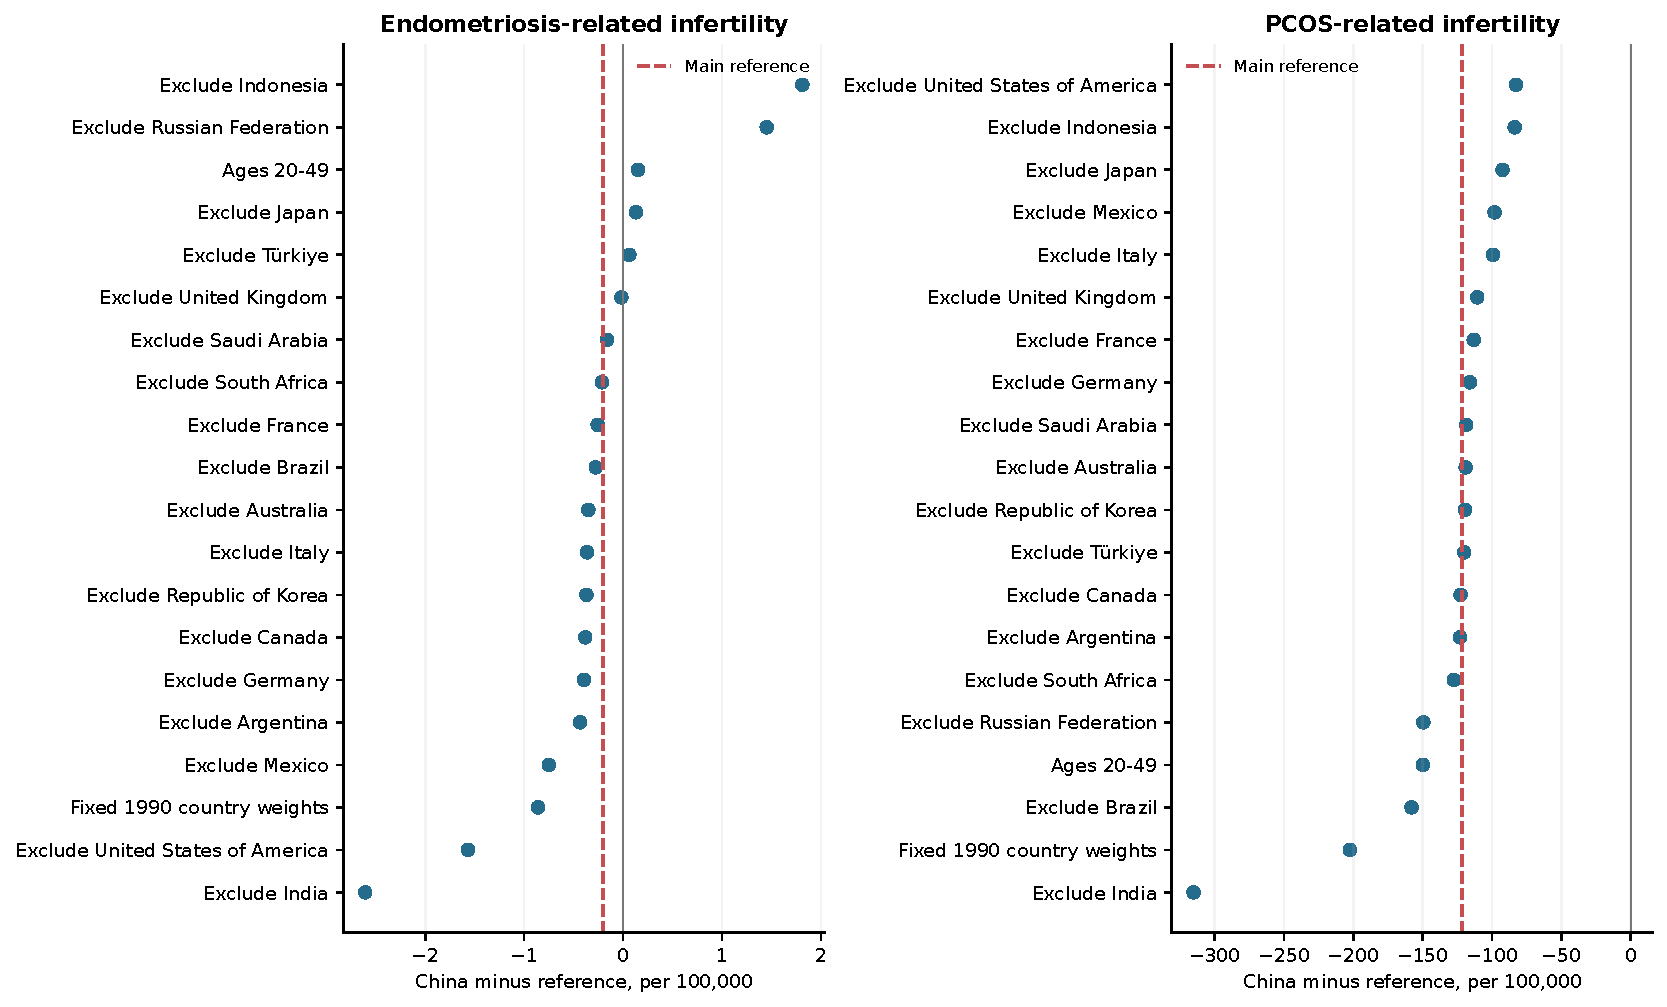
\includegraphics[width=\textwidth]{figures/figS1_reference_sensitivity.pdf}
\caption{Sensitivity of the 2023 prevalence difference to reference-country exclusions, fixed 1990 country shares within ages, and restriction to ages 20--49. Dashed lines show the main 15--49 comparison. PCOS signs are stable; endometriosis signs vary. All are point estimates.}\label{fig:sensitivity}\end{figure}
\begin{figure}[p]\centering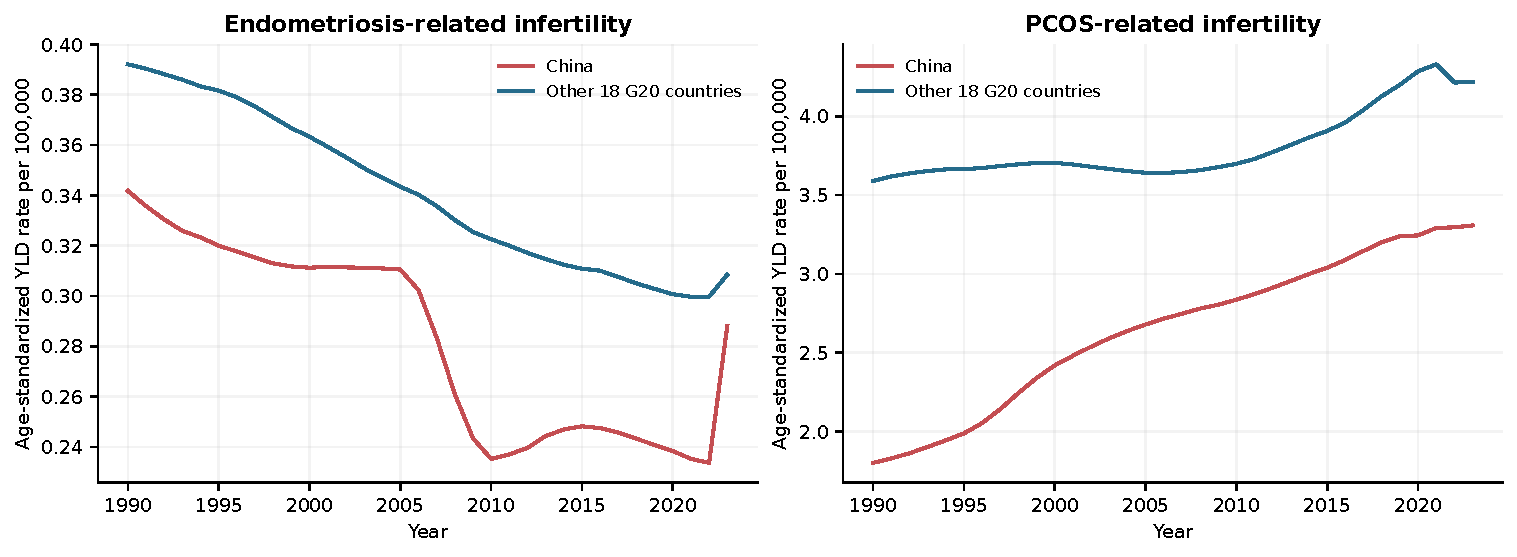
\includegraphics[width=\textwidth]{figures/figS2_yld_trends.pdf}
\caption{Restricted-age standardized YLD rates for both infertility causes, 1990--2023. These are infertility-impairment YLD rates rather than the total disability burden of either underlying disease.}\label{fig:yld}\end{figure}

\begin{figure}[htbp]\centering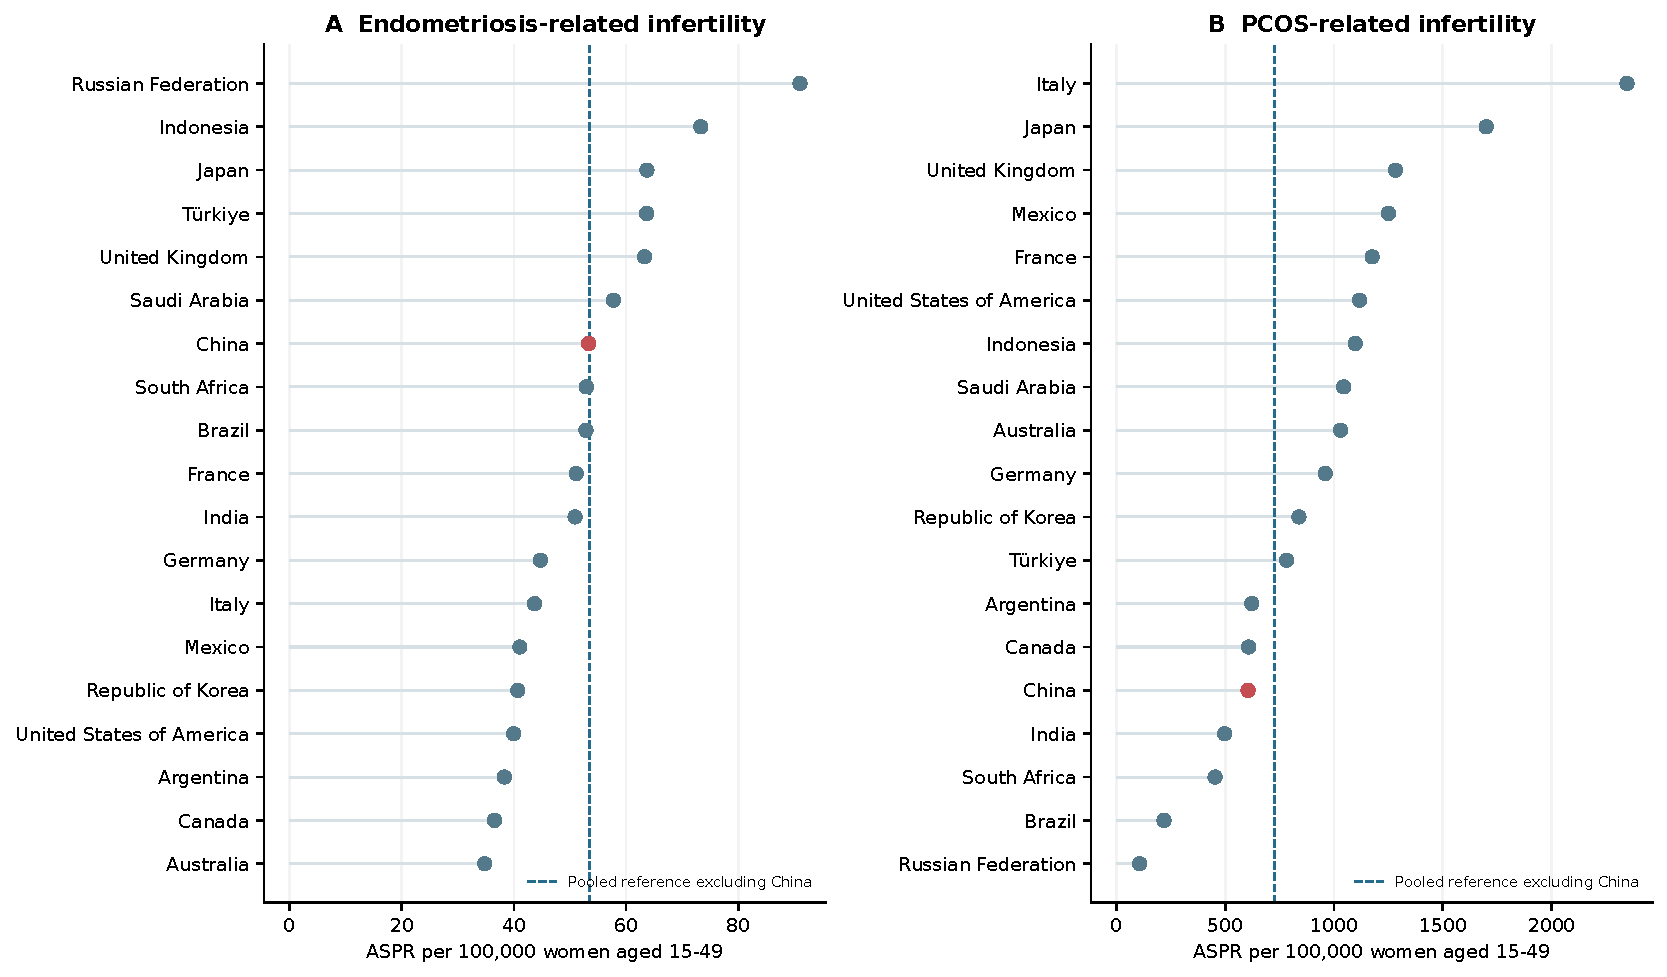
\includegraphics[width=\textwidth]{figures/fig1_country_comparison_2023.pdf}
\caption{Country-specific prevalence rates in 2023, restricted to ages 15--49. Dashed lines are the pooled reference. Descriptive point estimates only.}\end{figure}
\begin{figure}[htbp]\centering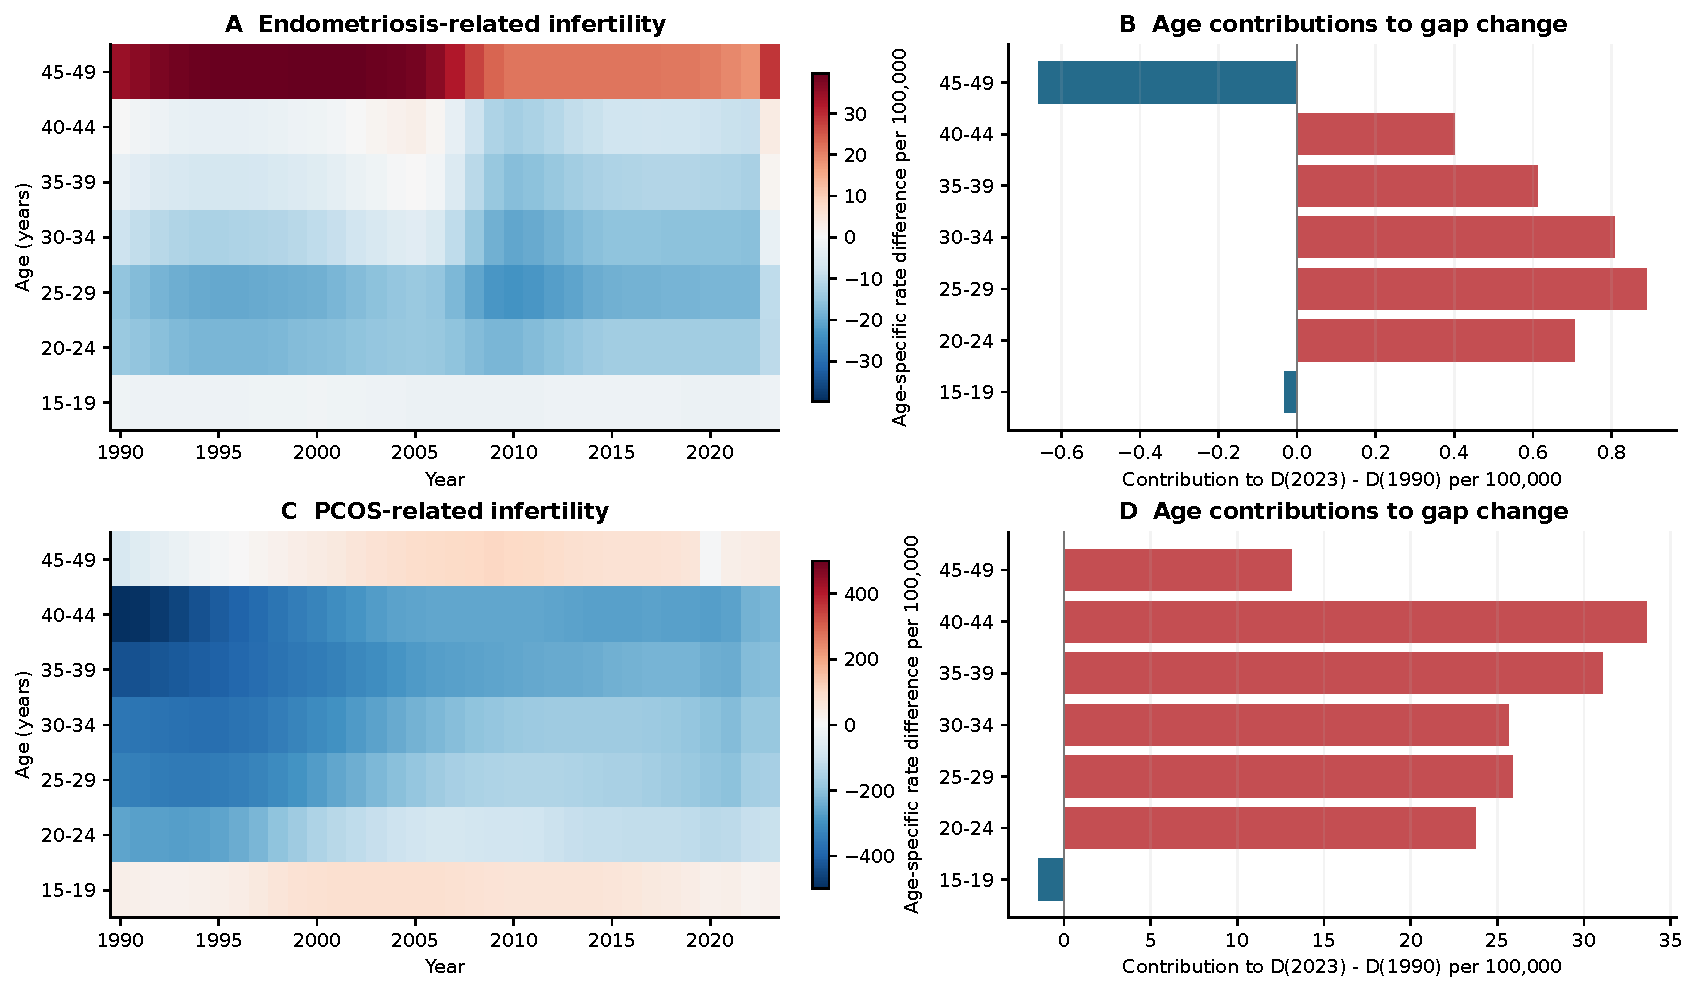
\includegraphics[width=\textwidth]{figures/fig3_age_disparities.pdf}
\caption{Age contrasts and standard-weighted contributions to changes in China minus reference. Contributions are not case counts or causal effects.}\end{figure}
\begin{figure}[htbp]\centering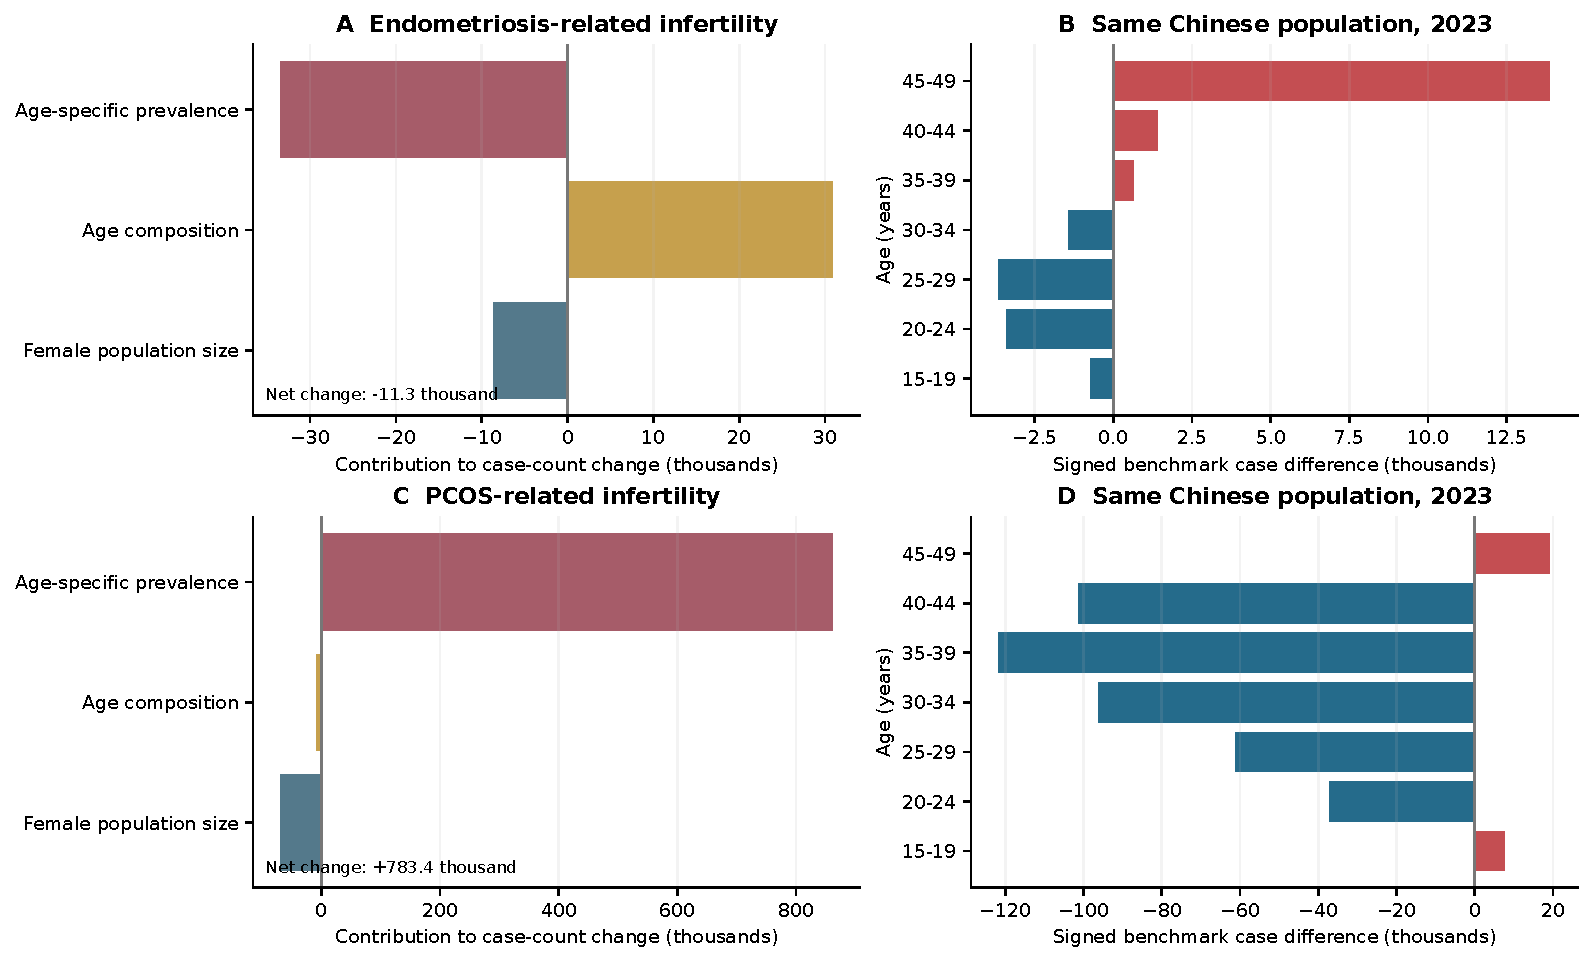
\includegraphics[width=\textwidth]{figures/fig4_decomposition_and_benchmark.pdf}
\caption{China's case-count decomposition and same-population benchmarks. The latter are signed arithmetic contrasts using China's actual age distribution, not preventable cases.}\end{figure}
\end{document}
